\documentclass[addpoints, 12pt]{exam}%, answers]
\usepackage[utf8]{inputenc}
\usepackage[T1]{fontenc}

\usepackage{lmodern}
\usepackage{arydshln}
\usepackage[margin=2cm]{geometry}

\usepackage{enumitem}
\usepackage{multicol}

\usepackage{enumerate}
\usepackage{breqn}
\usepackage{parskip}

\usepackage{amsmath, amsthm, amsfonts, amssymb}
\usepackage{graphicx}
\usepackage{tikz}
\usetikzlibrary{arrows,calc,patterns}
\usepackage{pgfplots}
\pgfplotsset{compat=newest}
\usepackage{url}
\usepackage{multicol}
\usepackage{thmtools}

\usepackage{caption}
\usepackage{subcaption}

\usepackage{pifont}

% MATH commands
\newcommand{\bC}{\mathbb{C}}
\newcommand{\bR}{\mathbb{R}}
\newcommand{\bN}{\mathbb{N}}
\newcommand{\bZ}{\mathbb{Z}}
\newcommand{\bT}{\mathbb{T}}
\newcommand{\bD}{\mathbb{D}}

\DeclareMathOperator{\dom}{dom}

\newcommand{\spc}{\vspace*{0.5cm}}
\CorrectChoiceEmphasis{\color{red}}

\begin{document}
\noindent \hrulefill \\
	MATH-241 Calculus I \hfill Created by Rukiyah Walker\\
	Homework 7 \hfill Spring 2023\\ \vspace*{-1cm}
 
	\noindent\hrulefill

\qformat{\rule{0.3\textwidth}{.4pt} \begin{large}{\textsc{Question}} \thequestion \end{large} \hspace*{0.2cm} \hrulefill \hspace*{0.1cm} \textbf{(\totalpoints\hspace*{0.1cm} pts)}}

\begin{questions}

\vspace*{0.5cm}

\question[1]

What is the main idea in a related rates problem?

\begin{choices}
\choice To find the average rate of change of a function $y$. 
\CorrectChoice To compute the rate of change of one quantity in terms of the rate of change of another quantity.
\choice To use the chain rule.
\choice To find the velocity of a particle at time $t$.
\end{choices}

\spc

\question[1]

\begin{minipage}{0.5\textwidth}
If $V$ is the volume of a cube with edge length $a$, and the cube expands over time, what is $\frac{dV}{dt}$? 

\begin{multicols}{2}
\begin{choices}
\choice $\frac{dV}{dt} = 3a^2$\vspace*{10pt}

\choice $\frac{dV}{dt} = a^3$\vspace*{10pt}

\CorrectChoice $\frac{dV}{dt} = 3a^2\frac{da}{dt}$\vspace*{10pt}

\choice $\frac{dV}{dt} = 3a$\vspace*{10pt}
\end{choices}
\end{multicols}
\end{minipage}
\hspace*{1cm}
\begin{minipage}{0.45\textwidth}
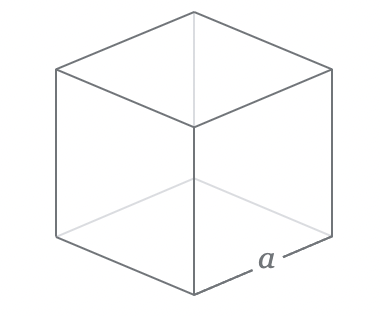
\includegraphics[width=0.75\textwidth]{HW7-cube.png}
\end{minipage}

\spc

\question[1]

Suppose you have the related rates problem: 

Each side of a square, labeled $x$, is increasing at a rate of $6m/s$. At what rate is the area of the square increasing when the area of the square is $16m^2$?

Identify what is given and what is unknown/the goal in the problem statement.

\begin{multicols}{2}
\begin{choices}
\choice Given: $\frac{dx}{dt}$.

Goal: $\frac{dx}{dt}$ at $x = 16 m^2$.
\choice Given: $\frac{dx}{dt}$.

Goal: $\frac{dA}{dt}$ at $x = 16 m^2$.
\choice Given: $\frac{dA}{dt}$.

Goal: $\frac{dx}{dt}$ at $x = 16 m^2$.
\CorrectChoice Given: $\frac{dx}{dt}$.

Goal: $\frac{dA}{dt}$ at $x = 4 m^2$.
\end{choices}
\end{multicols}

\newpage

\question[1]

Find the rate that the area of the square is increasing when the area is $16m^2$, from the \\Question 3.

\begin{multicols}{2}
\begin{choices}
\choice $192 m^2/s$
\CorrectChoice $48 m^2/s$
\choice $6 m^2/s$
\choice $32 m^2/s$
\end{choices}
\end{multicols}

\spc

\question[1]

Suppose $y = \sqrt{x^2 + 2x + 1}$, where $x$ and $y$ are \textbf{functions of $t$}. If $\frac{dx}{dt} = 3$, find $\frac{dy}{dt}$ when $x = 2$.

\begin{multicols}{2}
\begin{choices}
\CorrectChoice $\frac{dy}{dt} = 3$
\choice $\frac{dy}{dt} = \frac{1}{6}$
\choice $\frac{dy}{dt} = 2$
\choice $\frac{dy}{dt} = 9$
\end{choices}
\end{multicols}

\spc

\question[1]

When doing the process of linearization, we \textit{approximate} the values of the curve $y = f(x)$ by the tangent line at $(a, f(a))$, when $x$ is near $a$, if $f(x)$ is difficult to compute. Why can we do this?

\begin{choices}
\choice Since $f(a)$ is linearizable.
\choice The point of tangency exists.
\choice $f(x)$ is differentiable.
\CorrectChoice The curve $y = f(x)$ lies very close to it's tangent line near the point of tangency. 
\end{choices}

\spc

\question[1]

If $f(x) \approx f(a) + f'(a)(x-a)$, what is the linearization?

\begin{multicols}{2}
\begin{choices}
\choice $L(x) \approx f(a) + f'(a)(x-a)$
\choice $L(x) = f'(a)$
\CorrectChoice $L(x) = f(a) + f'(a)(x-a)$
\choice $L(x) = (x-a)'$
\end{choices}
\end{multicols}

\spc

\question[1]

Find the linearization $L(x)$ of $f(x) = x^3 -x^2 + 3$ at $a = -1$

\begin{multicols}{2}
\begin{choices}
\CorrectChoice $L(x) = 5x + 6$
\choice $L(x) = 16x + 23$
\choice $L(x) = 3x^2 - 2x$
\choice $L(x) = 5$
\end{choices}
\end{multicols}

\newpage

\question[1]

The differentiable $dy$ is the approximate increment in the variable $y$ given by $dy = f'(x)dx$. What is $dx$?

\begin{choices}
\choice An independent variable.
\choice The increment in the variable $x$.
\choice The differential of $x$.
\CorrectChoice All of the above.
\end{choices}

\spc

\question[1]

$dy$ represents the amount that the tangent line rises or falls when $x$ changes by an amount $dx$. What is this also known as?

\begin{choices}
\choice $\Delta y$
\CorrectChoice The change in linearization. 
\choice The change in $x$, $\Delta x$.
\choice $f'(x)$
\end{choices}

\end{questions}
\end{document}